\documentclass[a4paper]{article}

\usepackage{mathtools}
\usepackage{tikz}
\usetikzlibrary{automata,positioning,arrows,shapes,matrix}

\tikzset{
semithick,
node distance=1.5cm,
>=stealth,
initial text=,
every state/.style={draw,rectangle,rounded corners=2mm,inner sep=1mm,minimum height=2em}
}


\begin{document}

\begin{itemize} \itemsep3em
\item[] Initial automaton $\mathcal{A}$

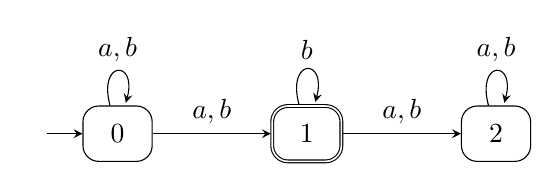
\begin{tikzpicture}
\node[initial,state]   (0)                {$0$};
\node[state,accepting] (1)  [right=of 0]  {$1$};
\node[state]           (2)  [right=of 1]  {$2$};

\path[->] (0)   edge[loop above]  node        {$a,b$}   ()
                edge              node[above] {$a,b$}   (1)
          (1)   edge[loop above]  node        {$b$}     ()
                edge              node[above] {$a,b$}   (2)
          (2)   edge[loop above]  node        {$a,b$}   ();
\end{tikzpicture}


\item[] Interim automaton $\mathcal{A}^\prime$ after subset-tuple construction on $\mathcal{A}$

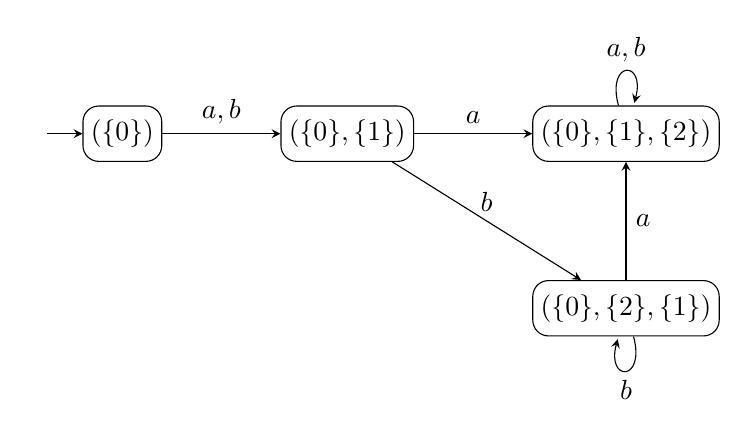
\begin{tikzpicture}
\node[initial,state] (0)                   {$\left(\{0\}\right)$};
\node[state]         (01)   [right=of 0]   {$\left(\{0\},\{1\}\right)$};
\node[state]         (012)  [right=of 01]  {$\left(\{0\},\{1\},\{2\}\right)$};
\node[state]         (021)  [below=of 012] {$\left(\{0\},\{2\},\{1\}\right)$};

\path[->] (0)   edge              node[above] {$a,b$} (01)
          (01)  edge              node[above] {$a$}   (012)
                edge              node[above] {$b$}   (021)
          (012) edge[loop above]  node        {$a,b$} ()
          (021) edge              node[right] {$a$}   (012)
                edge[loop below]  node        {$b$}   ();
\end{tikzpicture}

\end{itemize}

\end{document}